% Ubah kalimat sesuai dengan judul dari bab ini
\chapter{PROFIL PERUSAHAAN}
\vspace{4ex}

% Pengaturan ukuran indentasi
\setlength{\parindent}{7ex}

% Ubah konten-konten berikut sesuai dengan yang ingin diisi pada bab ini

\section{Sejarah PT. Aneka Tuna Indonesia}
\vspace{1ex}

PT. Aneka Tuna Indonesia berdiri pada didirikan pada bulan Oktober 1991, sebagai perusahaan gabungan antara Itochu Corporation dan Hagoromo Foods Corporation, yang merupakan pemilik merek tuna terkemuka di Jepang, serta satu perusahaan asing lainnya.
Terletak di daerah pegunungan dengan panorama eksotis di Provinsi Jawa Timur Indonesia, perusahaan ini mulai beroperasi secara  komersial pada bulan November 1992, mengkhususkan diri dalam produksi dan penjualan tuna kalengan.
\vspace{0.5ex}

Dalam praktiknya, Itochu melakukan penjualan dan manajemen keseluruhan, sementara Hagoromo Foods bertanggung jawab atas produksi.
Semua mitra secara aktif terlibat dalam peningkatan kualitas produk termasuk pengiriman teknisi dari Jepang dan pengiriman teknisi lokal ke Jepang untuk pelatihan.
\vspace{0.5ex}

\section{Visi dan Misi}
\vspace{1ex}

PT. Aneka Tuna Indonesia memiliki visi dan misi sebagai berikut:
\vspace{0.5ex}

\begin{enumerate}[nolistsep]

  \item \textbf{Visi PT. Aneka Tuna Indonesia}
  \vspace{0.5ex}

  Menjadi produsen tuna kaleng terkemuka di dunia.
  \vspace{0.5ex}

  \item \textbf{Misi PT. Aneka Tuna Indonesia}
  \vspace{0.5ex}

  \begin{enumerate}[nolistsep]

    \item Menjadikan semua stakeholder bagian penting dari perusahaan.
    \vspace{0.5ex}

    \item Menghasilkan produk yang berkualitas, sehat dan aman, serta ramah lingkungan.
    \vspace{0.5ex}

  \end{enumerate}
  \vspace{0.5ex}

\end{enumerate}
\vspace{0.5ex}

\section{Struktur Organisasi}
\vspace{1ex}

Struktur Organisasi dari PT. Aneka Tuna Indonesia adalah sebagai berikut.
\vspace{0.5ex}

% Contoh input gambar dengan format *.png
\begin{figure} [ht] \centering
  % Nama dari file gambar yang diinputkan
  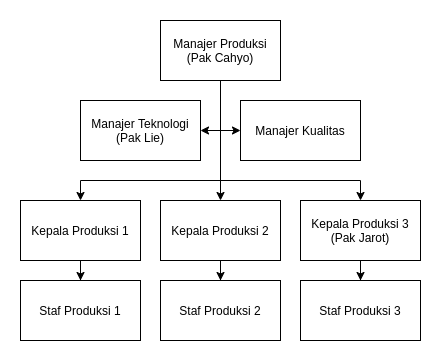
\includegraphics[width=0.95\textwidth]{gambar/hirarki-ati.png}
  % Keterangan gambar yang diinputkan
  \caption{Struktur Organisasi PT. Aneka Tuna Indonesia}
  % Label referensi dari gambar yang diinputkan
  \label{fig:strukturOrganisasi}
\end{figure}

% Contoh penggunaan referensi dari gambar yang diinputkan
Seperti yang bisa dilihat pada gambar \ref{fig:strukturOrganisasi}, Pabrik ATI 2 (Pabrik Pandaan) yang terletak di
Jl. Randupitu-Gunung Gangsir No.36, Asabri, Nogosari, Kec. Pandaan, Pasuruan, Jawa Timur dikepalai oleh seorang
manajer produksi yaitu pak Cahyo Prabowo. Dengan dibantu oleh dua subordinat yaitu manajer kualitas dan manajer
teknologi yang dijabat oleh pak Wie Sian Lie. Produksi pada Pabrik ATI 2 dibagi menjadi tiga bagian, yaitu Produksi 1,
Produksi 2, dan Produksi 3. Pada bagian Produksi 3 dikepalai oleh pak Jarot Wibowo Kusumo. Kepala Produksi 1, 2 , dan 3
membawahi staff yang sangat banyak (kurang lebih 3000 staff) yang terbagi menjadi beberapa tim dan juga shift kerja.
\vspace{0.5ex}
